\label{Chapter2}

\chapter{System Architecture}

\section{System Overview}

In order for planetary robots to navigate autonomously in extreme and
uncertain conditions where no GPS information is available,
they need to perceive their surroundings with high precision and
maintain this precision over time.
A way of compensating for the lack of real-time GPS data, is to use
an \textit{a priori} global map that contains 3D information about the
environment the robot is trying to navigate into.
This map can be reconstructed using imagery taken from an orbiter and
has a notably lower resolution compared to the robot's sensory data.
To take advantage of this existing information, we have developed a system
which is based around two layers of data processing.

In the first tier, the objective is to perceive the environment and
capture its 3D structure in order to enable the robot to navigate in it.
This is achieved by constructing a local map and estimating the robot's
current pose (position and orientation) w.r.t. its initial pose,
using sensory inputs and odometry data.
This process is commonly known as
\textit{Simultaneous Localization And Mapping} (SLAM) and can be expressed as
\begin{equation}
    p(x_{0:T} ,\ m_{1:T} \ | \ z_{1:T} ,\ u_{1:T})
\end{equation}
where
$x$ are the estimated poses of the robot,
$m$ is the constructed map of the environment,
$z$ are the sensory inputs and
$u$ are the robot's controls.
To reduce the problem's dimensions, the following factorization is performed
\begin{equation}
    p(x_{0:T} ,\ m_{1:T} \ | \ z_{1:T} ,\ u_{1:T}) =
    p(x_{0:T} \ | \ m_{1:T-1} ,\ z_{1:T} ,\ u_{1:T}) \
    p(m_{1:T} \ | \ x_{0:T} ,\ z_{1:T})
\end{equation}
where
the former belief represents the pose estimation problem, also called
relative localization, and the latter belief represents the mapping problem.

In the second tier, the objective is to achieve absolute localization by
eliminating the accummulated drift which occurs in the previous stage.
This drift is present in long-range scenarios and comes from the fact that
all the input information is coming directly from the robot itself.
To eliminate it, a matching technique is utilized in order to find the
position of the robot's local map inside a global map.

The separation of the system to two layers comes from the need to process the
data in separate moments, depending on the conditions of the environment as
well as on the robot's processing capabilities.
In Figure \ref{fig:HLD}, the high-level design diagram of the system shows
the 4 main modules that comprise the entire system.
Their functionality is explained in the following sections of this chapter.

\begin{figure}[th]
    \centering
    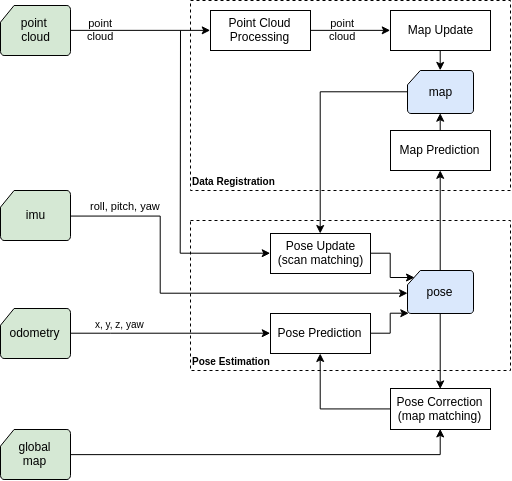
\includegraphics[scale=0.4]{Figures/high_level_design_diagram}
    \decoRule
    \caption[High Level Design Diagram]{
        The high-level design diagram showing the submodules that comprise
        the system as well as the data flow.}
    \label{fig:HLD}
\end{figure}

\section{Data Registration}

An integral aspect of a robotic system, is the mapping process.
The map is the model of the environment and can represent information about
it in either two or three dimensions.
In addition, the information a map represents can be organized either in
a grid-based manner (volumetric map) or in the form of landmarks
(feature-based map).
Volumetric maps provide a more detailed and precise model of the environment
compared to feature-based maps and are, therefore, the better choice for
robots that aim to solve navigation tasks.
Moreover, autonomous robots that need to navigate in non-flat surfaces,
require a 3D model in order to safely avoid the terrain's obstacles.
Robotic applications with this requirement include outdoor, underwater,
airborne or planetary missions.

% TODO(ref): mapping and classification

As we have already mentioned, planetary rovers have an important constraint
in on-board computational power.
This limitation deems the use of pure 3D maps inappropriate.
To overcome this problem, we can represent the environment with a 2.5D map,
known as elevation map.
An elevation map is essentially a 2D grid-map composed of cells that hold
the value of the terrain's elevation.
It is important to note that this mapping method does not model completely
the 3D environment, but can provide a sufficient approximation even for
the most demanding applications.

% TODO(ref): elevation map

To make use of this mapping technique, a robot must be equipped with a
sensor that is capable of providing measurements in the 3D space.
Such measurements are usually stored in a structure called point cloud -
a set of points $P$ that contain information about their position in
space $(x,y,z)$.
A point cloud can be constructed from sensors that provide depth information,
with the most popular being stereo cameras, time-of-flight (ToF) cameras
and LiDARs.

% TODO(ref): point cloud

In this section, the functionality of the Data Registration module will be
explained.
Its main purpose is to preprocess the input sensor data (point cloud)
and register it to create an elevation map or update an existing one.

\subsection{Point Cloud Preprocessing} \label{point_cloud_processing}

The importance of preprocessing a point cloud before registering its data
in a map, comes from the fact that point clouds contain large amount of points
and hence process them is a time-consuming task.
Additionally, the points represented in the cloud may be referenced in a
different frame (usually the sensor's frame) than the frame of the map.

For this purpose, we implemented a point cloud preprocessing submodule,
that consists of the following four steps:

\begin{enumerate}
    \item \textbf{Voxelization}:
        In this step, we reduce the volume of the point cloud by downsampling
        it using a discrete 3D grid.
        Each cell of the grid, called \textit{voxel}, is mapped to $\{0,1\}$
        and it therefore represents the existence or absence of an obstacle
        in that position.
        This method is called \textit{voxelization} and results in a more
        sparse cloud of 3D points.
        % However, the larger the voxels are, the less precise the
        % representation of the space becomes.

        % TODO: Add equation for voxelization
        % TODO(ref): voxelization

    \item \textbf{Transformation}:
        A point $P$ sampled from the sensor is in the sensor's reference frame
        $S$ and need to be transformed in the map's frame $M$ in order to be
        registered.
        This is be achieved by
        \begin{equation}
            \mathbf{t}_{MP} =
                \mathbf{R}_{SM} \mathbf{t}_{SP} -
                \mathbf{t}_{SM}
        \end{equation}
        where
        $\mathbf{t}_{MP}$ is the position of $P$ in the map frame,
        $\mathbf{t}_{SP}$ is the position of $P$ in the sensor frame,
        $\mathbf{R}_{SM}$ is the rotation between the sensor frame and the
        map frame and
        $\mathbf{t}_{SM}$ is the translation between them.

    \item \textbf{Cropping}:
        Since a point cloud can span a wide area in space depending on the
        sensor's field of view and orientation, we can further reduce the
        volume of the cloud by discarding (cropping) points that fall out
        of the map.
        This is done by defining a box in space and removing
        from the point set all the points that are not inside it.
        In our case, we define the minimum and maximum cutoff points that
        represent the diagonal of the crop box as
        \begin{equation}
        \begin{aligned}
            &min\_cutoff\_point =
                \left( \
                    - \frac{l_x}{2} - t_x, \
                    - \frac{l_y}{2} - t_y, \
                    z_{min} \
                \right) \\
            &max\_cutoff\_point =
                \left( \
                    \frac{l_x}{2} + t_x, \
                    \frac{l_y}{2} + t_y, \
                    z_{max} \
                \right)
        \end{aligned}
        \end{equation}
        where
        $l_x$ and $l_y$ are the lengths of the map in meters in the
        x and y axis,
        $t_x$ and $t_y$ are the positions of the map in meters in the
        x and y axis and
        $z_{min}$ and $z_{max}$ are the minimum and maximum elevation
        of the map.

    \item \textbf{Uncertainty calculation}:
        In this last step, we use the sensor's model to calculate the variance
        of each point in the point cloud, $\sigma^2_z$.
        As a result, each point will contain in addition to a $x$ and $y$
        position, a one-dimensional Gaussian distribution for the height.
        This calculation is different for every sensor, since it depends
        on the sensor's characteristic.
        For a stereo camera, we approximate the variance as
        \begin{equation}
            \sigma^2_z = \dots
        \end{equation}
\end{enumerate}

% TODO: Add figure of point cloud pre and post processing

\subsection{Registration}

\subsubsection{Structure of Elevation Map} \label{map_structure}

The elevation map, also referred to as \textit{local map} or simply
\textit{map}, is a robot-centric grid-based map.
This means that it is centered in the robot's position in the
global reference frame.
When the robot moves, previous cells that now fall out of the map are
reset and values that belong to the new explored area take their place.

The map models the elevation of the environment as well as the uncertainty
of it.
As a result, in every position of the 2D grid, the elevation is
represented by a one-dimensional Gaussian distribution.
This means that the the map consists of two layers

\begin{itemize}
    \item the layer of \textit{mean} elevation $(\mu_z)$ and
    \item the layer of elevation \textit{variance} $(\sigma^2_z)$
\end{itemize}
% TODO: Add the two translation variance layers

Apart from its structure, a map is also characterized by a few other
properties.
The most important are

\begin{itemize}
    \item the \textit{resolution}, which is the dimension of a cell in meters,
    \item the \textit{length}, which is the length of the map in meters,
    \item the \textit{minimum} and \textit{maximum} elevation values that
        the map can hold,
    \item the 2D \textit{position} of the map in the global reference frame and
    \item the \textit{orientation} of the map in the global reference frame
\end{itemize}

Regarding the last property, it is worth mentioning that the orientation
of the map is fixed w.r.t. to the global frame.
This decision was made in order to reduce the complexity when performing
a prediction of the map (see next section).

\subsubsection{Map Prediction and Update} \label{map_prediction_and_update}

Even though the map prediction and update steps are grouped in the
same submodule, they implement two separate functionalities.
The map prediction is triggered when a new odometry pose is received and
processed by the Pose Estimation module (Section \ref{pose_estimation}).
The map update is triggered as soon as a new point cloud arrives from
the sensor.
\begin{itemize}[listparindent=1.5em]
    \item \textbf{Prediction} \\
        This step is responsible for moving the map when the robot assumes
        a new position.
        This is essentially a simple 2D transformation of the map's position
        in the $x$ and $y$ axes.
        The robot's orientation is not taken into account, since as we said
        earlier (Section \ref{map_structure}), the orientation of the map
        about the $z$ axis is fixed.
        To perform the prediction, we simply

        \begin{enumerate}
            \item apply the delta translation $(t_x,t_y)$ of the
                new estimated pose to map and
            \item keep the height Gaussian $(\mu_z,\sigma^2_z)$ of
                each cell unchanged
        \end{enumerate}

        When a translation is applied to the map, cells that fall out of the
        map have their values reset and elevation values of the new explored
        area take their place instead.
        To avoid unnecessary data copying in memory, the data storage can be
        implemented as a two-dimensional circular buffer.

    \item \label{map_update} \textbf{Update} \\
        This is the core step of the Data Registration module, since this
        step implements the registration of the input point cloud into the map.
        The algorithm of the point cloud projection is shown in Algorithm
        \ref{alg:map_update}.

        It uses a probabilistic approach to take advantage of the
        fact that both the point cloud (Section \ref{point_cloud_processing})
        and the map (Section \ref{map_structure}) represent the elevation
        as a one-dimensional Gaussian distribution.
        The last operation of the algorithm (Operation \ref{op:fuse}) is the
        actual fusion, and can be implemented with different methods.
        A popular method is the one used in a Kalman filter, which given
        two Gaussian distributions $N(\mu_1, \sigma^2_1)$ and
        $N(\mu_2, \sigma^2_2)$, can be implemented as
        % TODO(ref): kalman filter sensor fusion (see elevation mapping paper)

        \begin{equation}
            innovation = \mu_2 - \mu_1
        \end{equation}
        \begin{equation}
            gain = \frac {\sigma^2_1} {\sigma^2_1 + \sigma^2_2}
        \end{equation}
        \begin{equation}
            \mu_1 = \mu_1 + gain \cdot innovation
        \end{equation}
        \begin{equation}
            \sigma^2_1 = \left( 1 - gain \right) \cdot \sigma^2_1
        \end{equation}

        \begin{algorithm}
            \caption{Registration of point cloud to map}
            \label{alg:map_update}
            \begin{algorithmic}[1]
                \State $map$: two-dimensional grid of $\{\mu_z, \sigma^2_z\}$
                \State $point\_cloud$: set of $\{x, y, z\}$
                \State $point\_cloud\_variances$: set of $\{\sigma^2_z\}$ \\

                \For {every $point$ in the $point\_cloud$}
                    \If {$point$ is outside of the $map$}
                        \State \textbf{continue}
                    \EndIf \\

                    \Let {$point\_mean$} {$point[z]$}
                    \Comment projection of the point
                    \Let {$point\_variance$} {$point\_cloud\_variances
                        [point\_index]$} \\

                    \Let {$index$} {$find\_map\_index(point[x], point[y])$}
                    \Comment corresponding cell in grid
                    \Let {$cell\_mean$} {$map[mean][index]$}
                    \Let {$cell\_variance$} {$map[variance][index]$} \\

                    \If {$cell\_mean$ or $cell\_variance$ is not initialized}
                        \Let {$cell\_mean$} {$point\_mean$}
                        \Let {$cell\_variance$} {$point\_variance$}
                    \Else
                        \State $fuse(cell\_mean, cell\_variance,
                            point\_mean, point\_variance)$ \label{op:fuse}
                    \EndIf \\

                    \Let {$map[mean][index]$} {$cell\_mean$}
                    \Let {$map[variance][index]$} {$cell\_variance$}
                \EndFor
            \end{algorithmic}
        \end{algorithm}
\end{itemize}

% TODO: add figures of input point cloud and its projection in the map

\section{Data Fusion}

The goal of this module is to fuse data from different sources and
increase the overall quality of the map.
This is achieved by taking advantage the already computed uncertainty
estimates in the map and applying fusion techniques to improve the
existing data.
In particular, we developed two submodules to perform fusion in separate
stages of the pipeline.
These are explained in the following sections.

\subsection{Sensor Fusion}

Using sensor fusion we can exploit the multiple sensors equipped in
a robot to increase the covered area in the map.
In addition to increased coverage, fusing sensor data that are overlapping
in the map can increase its quality.

The way a point cloud is registered (fused) in the map, was already mentioned
in a previous section (Section \ref{map_update}).
Using this method we can combine information from different sensors, as long
as the input data is in the form of a point cloud, by simply updating the map
and taking advantage of the uncertainty estimates that are calculated
in the preprocessing of the point cloud.

% TODO: Add figures of point clouds from different sensors and the resulting map from fusion

A drawback of this technique is that large calibration errors and inaccuracies
in the transformations $(\mathbf{t}_{SM}$ and $\mathbf{R}_{SM})$ between a
sensor and the map can have the opposite effect i.e. deteriorate the map
quality.
This is due to the fact that fusion can over-smooth obstacles
since their correspondence in the map will be slightly different
for each sensor.
Errors like these can easily produce false negative obstacles and
have a detrimental effect in the navigation of the robot.

% TODO: Add figure illustrating this point

% \subsection{Neighborhood Fusion}

% Explain what is neighborhood fusion and the steps
    %\item increase map quality using the translation uncertainties

% \bigskip
% \noindent
% For each cell of map:
% \begin{enumerate}
%     \item Compute a weight for every neighboor cell according to distance/variance
%     \item Update mean/variance of cell using a weight-based fusion rule
% \end{enumerate}

% \noindent
% Add equation for the weight calculation and the fusion rule\\
% If visible, add figures showing the variance layers in the map, and the result of the fusion (prior and posterior mean elevation layers)

\section{Pose Estimation} \label{pose_estimation}

The pose, or state, of a robot navigating in a 3D environment, consists of
its position $(x, y, z)$ and its orientation $(roll, pitch, yaw)$ w.r.t.
a global reference frame.
Hence, the goal of pose estimation, also referred to as relative localization,
is to accurately track the robot's pose in the environment.
This is usually accomplished by either employing a probabilistic filter,
e.g. a Kalman filter or a particle filter, or by utilizing methods such
as scan matching.
A filter's inputs are usually expressed in the form of position or velocity
and can be extracted using odometry techniques.
In comparison, the input of a scan matching method is by definition a
scan, i.e. measurement, received by a sensor.
% TODO(ref): filtering / scan matching
For our case, we approached the localization problem by making use of a
combination of scan matching and particle filtering techniques.

First, we assume the state of the problem to be
\begin{equation}
    \mathbf{x} =
    {[x \quad y \quad z \quad roll \quad pitch \quad yaw]}^\intercal
\end{equation}
where $roll$, $pitch$ and $yaw$ are the rotations about the $x$, $y$ and $z$
axes respectively.
However, we cannot obtain accurate estimates for the $roll$ and $pitch$ states
from odometry.
To overcome this limitation, we use an \textit{inertial measurement unit} (IMU)
sensor and receive these states directly from it, so the problem state becomes
\begin{equation}
    \mathbf{x} = {[x \quad y \quad z \quad yaw]}^\intercal
\end{equation}
By making the assumption that the $z$ estimation from odometry is accurate
in an area near the robot, the state can be further simplified as
\begin{equation}
    \mathbf{x} = {[x \quad y \quad yaw]}^\intercal
\end{equation}
In the case where this assumption is false, the result will be a deformed
map, since the elevation values of the map will be directly affected
by the wrong $z$ estimate of the robot.

To estimate the posterior of the robot state, a particle filter is employed,
that samples particles in a continuous state space.
Additionally, the uncertainty of each particle is modelled using
a Gaussian distribution.

where the
the odometry inputs are used to predict the state of each particle and
the sensory inputs, i.e. point clouds, are used for the weight update.

Finally, $yaw$ measurements from the robot's IMU sensor are fused with the
final estimate to provide more accurate measurements.

% TODO: add a figure showing the particle distribution around the robot
% TODO: add a figure showing the 3D pose estimation compared to ground truth

An activity diagram illustrating the algorithm's steps is shown in Figure X.
These steps are explained in detail in the following sections.

% TODO: add pose estimation activity diagram

\subsection{Initialization}

Explain the step

\begin{enumerate}
    \item Sample all particles at initial pose
\end{enumerate}

\noindent
Add gaussian sampling equation

\subsection{Prediction}

Explain the steps

\begin{enumerate}
    \item Add gaussian noise to delta pose transformation from visual odometry
    \item Apply transformation to each particle
\end{enumerate}

\noindent
Add prediction equations (trivial)

\subsection{Update}

Explain the steps

\begin{enumerate}
    \item Crop local map to sensor's dimensions
    \item Create point cloud from local map
    \item Crop raw (input) cloud to map size
    \item Downsample raw and map point clouds (for faster convergence of point cloud alignment)
    \item For each particle
        \begin{enumerate}
            \item Create particle point cloud by transforming map point cloud to particle's pose
            \item Measure particle and raw point cloud alignment using mean square error
            \item Assign inverse error as particle's weight
        \end{enumerate}
\end{enumerate}

\noindent
Add equations of point cloud alignment method for the weight update

\subsection{Resampling}

Explain the technique used, the steps and the strategy

\begin{itemize}
    \item Technique: multinomial resampling
    \item Steps
        \begin{enumerate}
            \item Normalize particle weights to form cummulative distribution
            \item Sample uniformally each particle from cummulative distribution
            \item Strategy: resample every X filter updates, depending on the robot's speed and the particle scattering (noise)
        \end{enumerate}
\end{itemize}

\noindent
Add equations for forming and sampling from the cummulative distribution

\subsection{Estimation}

Explain the steps

\begin{enumerate}
    \item Estimate pose from particle cloud:
        \begin{enumerate}
            \item Ignore particles with weights below a specific threshold
            \item Pick top X particles
            \item Calculate new estimate by performing a weighted average of particles
            \item Calculate pose variance from the distribution of the particle cloud
        \end{enumerate}
    \item Fuse IMU/Odometry states:
        \begin{enumerate}
            \item Get roll and pitch measurements directly from the IMU
            \item Get z estimation directly from visual odometry
            \item Fuse IMU (laser gyroscope) yaw measurement with the PF's yaw estimate by means of 1D gaussian fusion
        \end{enumerate}
\end{enumerate}

\noindent
Add equations for calculating the mean and the variance values of the estimate\\
Mention that the robot's absolute z estimate is not of importance and why is that

\section{Pose Correction}

Explain what is the purpose of this step\\
Explain the execution strategy of this step\\
Mention known limitations of this approach

\begin{itemize}
    \item Purpose: to minimize absolute localization drift using the global map
    \item Strategy:
        \begin{itemize}
            \item Generic: map needs to have features \& robot must have covered certain amount of cells in the global map
            \item Planetary specific: correct pose by the end of the day (for energy efficience reasons)
        \end{itemize}
    \item Limitations:
        \begin{itemize}
            \item When there are no features, the local to global map matching will fail
            \item For safety purposes, the rover tries to generate a global path (using the global map) with as few features (i.e. rocks/craters) as possible
        \end{itemize}
\end{itemize}

\subsection{Global to Local Map Matching}

Explain the steps\\
Explain why a template matching method is used instead of a feature-based one

\begin{enumerate}
    \item Downsample local map to match global map's resolution
    \item Calculate gradient (magnitude of the edge) of local and global map's elevation values
    \item Replace unknown cell values with zero (does not affect matching)
    \item Warp the local map to specific yaw angles to find a yaw correction
    \item For each yaw angle: match local map to global map using template matching with normalized correlation coefficients
 Select or discard best match if score is above X (e.g. 95\%)
    \item Convert the matched position from image coordinates to map coordinates
    \item Add gaussian noise to delta transformation (x \& y) from matching
    \item Apply transformation to each particle of particle filter
\end{enumerate}

\noindent
Add figures of:
\begin{itemize}
    \item comparing Sobel edges with Scharr/Laplacian to justify the method
    \item source global/local maps in the scene (3D)
    \item source global/local maps in 2D
    \item downsampled local map
    \item gradients of global/local maps
    \item result image of matching with rectangles indicating the match \& the ground truth match
\end{itemize}

\noindent
Add equations of:
\begin{itemize}
    \item nearest neighbor method for downsampling the local map
    \item gradient calculations (sobel kernel etc.)
    \item template matching method (normalized correlation coefficients)
    \item selection technique of best position from result image
\end{itemize}

\subsection{Criteria Checking}

\subsubsection{Elevation Features Checking}

Explain the steps and the threshold parameter selection

\begin{enumerate}
    \item Create slope map from local elevation map by calculating the elevation gradient
    \item Remove values in slope map below a specific threshold
    \item Add remaining values to get absolute slope of map
    \item Compare to threshold
\end{enumerate}

\noindent
Add equation for calculating the gradient and thresholding the map (image)\\
Add figures of final slope maps that succeed/fail the criterion

\subsubsection{Traversed Distance Checking}

Explain the step and the threshold parameter selection

\begin{enumerate}
    \item Calculate traversed distance since last pose correction step
    \item Compare to threshold
\end{enumerate}

\noindent
Add equation for the distance calculation (very trivial)\\
Add figures of robot traverses that succeed/fail the criterion

